\documentclass[aspectratio=43,11pt,xcolor={dvipsnames}]{beamer}
\usetheme{Madrid}
\usecolortheme{seahorse}
\usefonttheme{serif}
\usepackage[utf8]{inputenc}
\usepackage{amsmath}
\usepackage{amsfonts}
\usepackage{amssymb}
\usepackage{algorithm}
\usepackage{algpseudocode}
\hypersetup{pdfpagemode=FullScreen}
\usepackage{calc}
\usepackage[normalem]{ulem}% to striketrhourhg text
\usepackage{subcaption}
\usepackage{caption}
\captionsetup[figure]{labelformat=empty}% we don't need 'Figure' lable
\usepackage{smartdiagram}
\usesmartdiagramlibrary{additions}

\usepackage[style=verbose,backend=bibtex]{biblatex}
\renewcommand*{\bibfont}{\tiny}%font size for reference slide
\addbibresource{bibfile.bib}

\setbeamertemplate{navigation symbols}{}
\renewcommand{\footnotesize}{\tiny}

\title[AIR 2017]{Robotic cloth manipulation for clothing assistance task using Dynamic Movement Primitives}
\author[Ravi P. Joshi]{Ravi P. Joshi$^a$, Nishanth Koganti$^{a,b}$, and Tomohiro Shibata$^a$}
\institute[]{\tiny{$^a$Graduate School of Life Science and Systems Engineering, Kyushu Institute of Technology, Kitakyushu, Japan\\$^b$Graduate School of Information Science, Nara Institute of Science and Technology, Nara, Japan}}

\date[]{{June 29, 2017}}

% all the graphics are placed inside images folder
\graphicspath{{./images/}}

\titlegraphic{
\includegraphics[scale=0.08]{kyutech} \hskip1cm 
\includegraphics[scale=0.08]{naist}}

%src: https://tex.stackexchange.com/a/248147
\defbeamertemplate{title page}{noinstitute}[1][]
{
  \vbox{}
  \vfill
  \begingroup
    \centering
    \vskip3em\par
    \begin{beamercolorbox}[sep=4pt,center,#1]{title}
      \usebeamerfont{title}\inserttitle\par%
      \ifx\insertsubtitle\@empty%
      \else%
        \vskip0.1em%
        {\usebeamerfont{subtitle}\usebeamercolor[fg]{subtitle}\insertsubtitle\par}%
      \fi%
    \end{beamercolorbox}%
    \vskip0em\par
    \begin{beamercolorbox}[sep=8pt,center,#1]{author}
      \usebeamerfont{author}\insertauthor
    \end{beamercolorbox}
    \begin{beamercolorbox}[sep=8pt,center,#1]{institute}
      \usebeamerfont{date}\insertinstitute
    \end{beamercolorbox}\vskip0.1em
    \begin{beamercolorbox}[sep=8pt,center,#1]{date}
      \usebeamerfont{date}\insertdate
    \end{beamercolorbox}\vskip0.1em
    {\usebeamercolor[fg]{titlegraphic}\inserttitlegraphic\par}
  \endgroup
  \vfill
}

\makeatletter
\setbeamertemplate{title page}[noinstitute][colsep=-4bp,rounded=true,shadow=\beamer@themerounded@shadow]
\makeatother

\begin{document}
{
	\usebackgroundtemplate{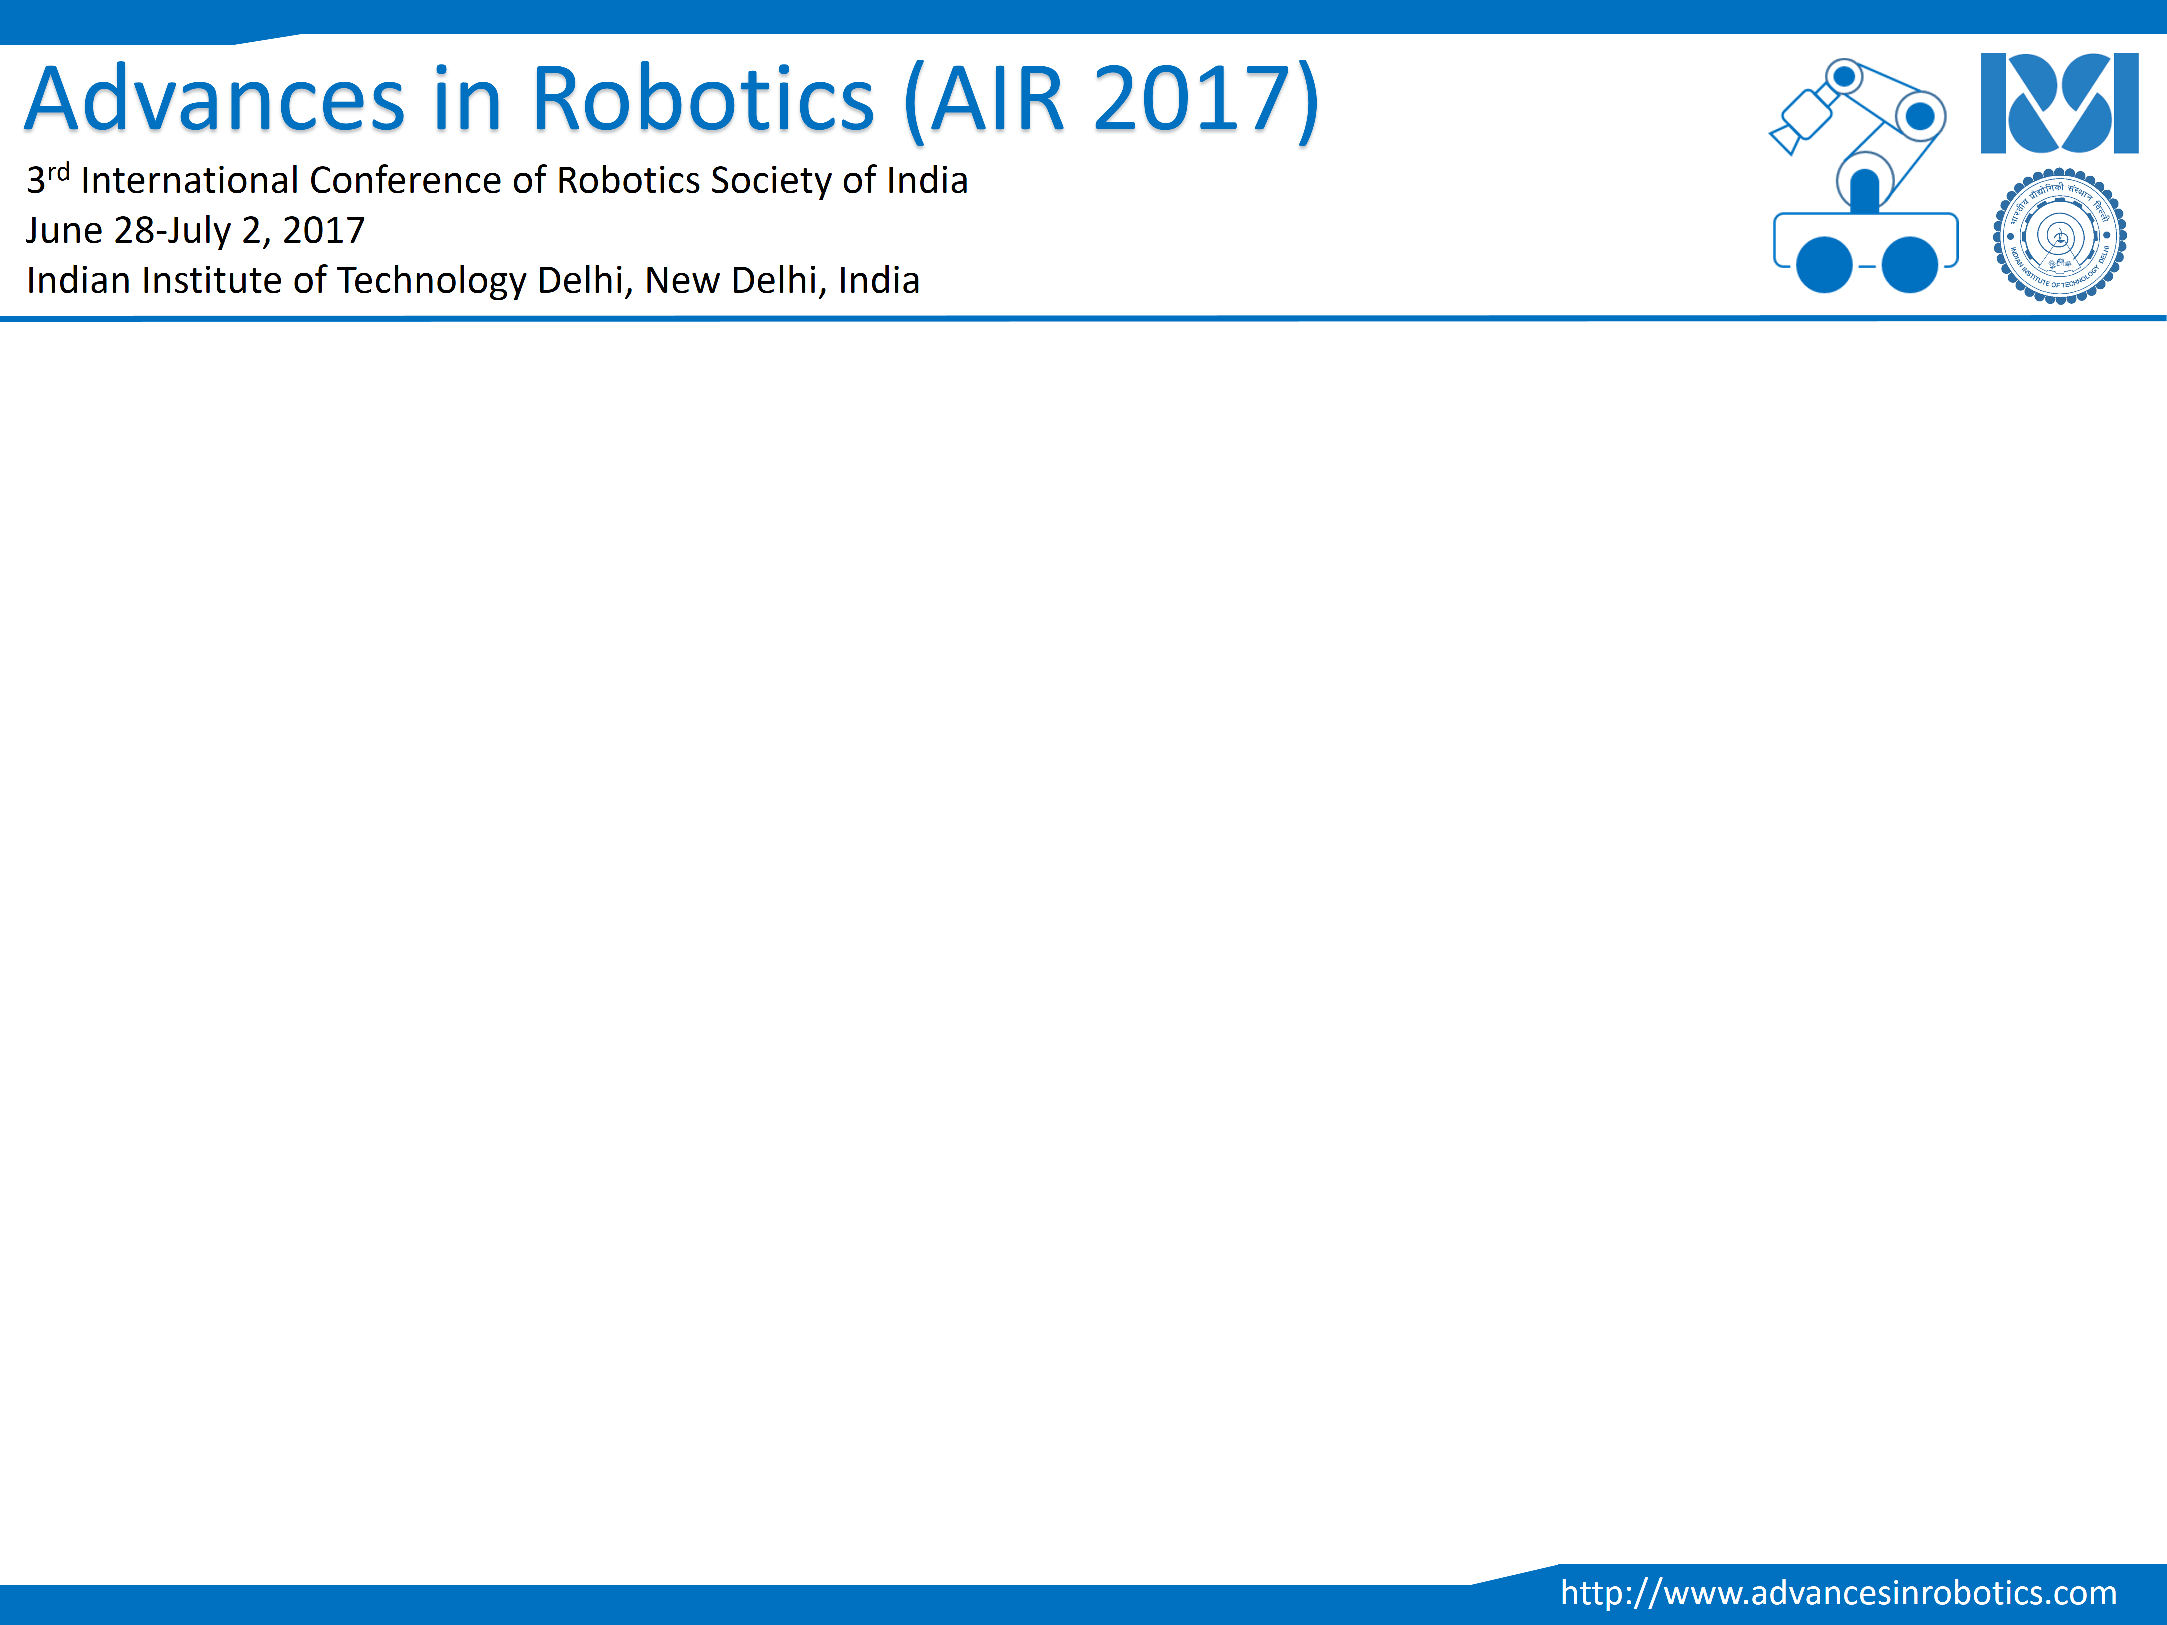
\includegraphics[width=\paperwidth]{background}}
	\setbeamertemplate{footline}{}
	\begin{frame}
		\titlepage
	\end{frame}
}
\addtocounter{framenumber}{-1}

%\begin{frame}[noframenumbering]
%	\titlepage
%\end{frame}

%\begin{frame}[noframenumbering,label=main]{Outline}
%	\tableofcontents
%\end{frame}

\section{Introduction}
\begin{frame}{Introduction}
	%\linespread{1.5}
	
	\vskip -2em
	\begin{columns}[t]
		\begin{column}{0.6\textwidth}
			\begin{itemize}
				\item Japan is a super-aging society
				\item In 2030, 1.8 person is supposed to care 1 elderly
				\item 400,000 care givers are lacking now
				\item Clothing is one of the most suffering daily activities for elderly
			\end{itemize}
		\end{column}
								
		\begin{column}{0.4\textwidth}
			\vskip -1em
			\begin{figure}
				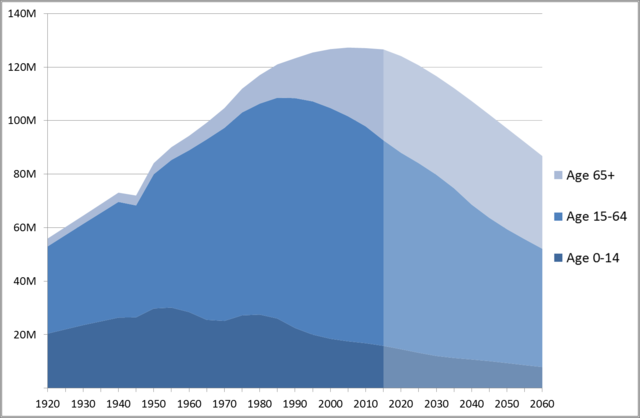
\includegraphics[trim={4px 4px 4px 4px},clip,width=\textwidth]{japan_population}
				\caption{Japan population growth\footnotemark}
			\end{figure}
		\end{column}
	\end{columns}
				
	\vskip -1em
	\begin{columns}[t]
		\begin{column}{0.7\textwidth}
			\begin{block}{Major challenges involved}
				\begin{itemize}
					\item Close interaction of the robot with cloth
					\item Safe human-robot interaction
					\item Estimation of human-cloth relationship
				\end{itemize}
			\end{block}
		\end{column}
								
		\begin{column}{0.25\textwidth}
			\begin{figure}
				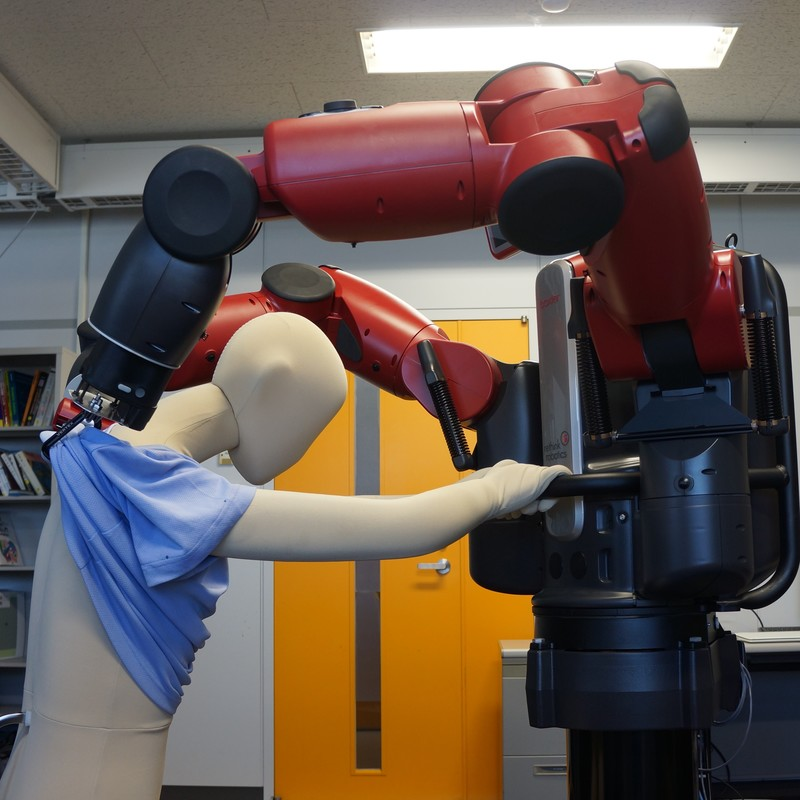
\includegraphics[width=0.7\textwidth]{robotic_clothing_assistance}
			\end{figure}
		\end{column}
	\end{columns}
	
	\footcitetext{jonMcDonald2016japan}
\end{frame}

\section{Related Works}
\begin{frame}{Related Works}
				
	\vskip -1em
	\begin{columns}[t]
		\begin{column}{0.5\textwidth}
			Towner \textit{et al.}\footnotemark, ~Manipulating clothing article by dual-arm robot
			{\scriptsize
				\begin{itemize}
					\item Used Hidden Markov Model for tracking
					\item Triangulated mesh model for simulating clothing article
					\item Highly depends on simulated contour information.
				\end{itemize}
			}
			\vskip 0.5em
			\centering{
				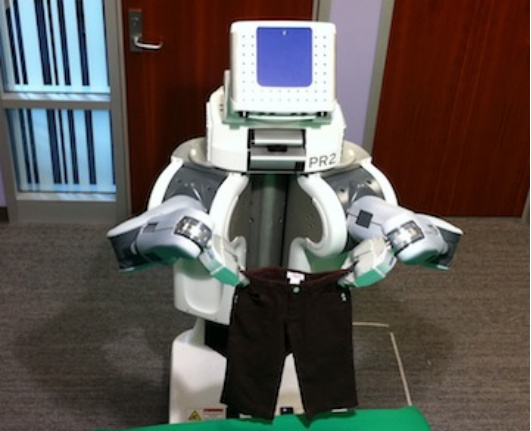
\includegraphics[height=2.5cm]{towner_2011}
			}
		\end{column}
								
		\begin{column}{0.5\textwidth}
			Tamei \textit{et al.}\footnotemark, ~Clothing assistance with dual-arm robot
			{\scriptsize
				\begin{itemize}
					\item Used Reinforcement learning (RL)
					\item Topology coordinates for human and cloth extremities relationship
					\item Via-point trajectory with minimum jerk criterion
				\end{itemize}
			}
			\vskip 0.5em
			\centering{
				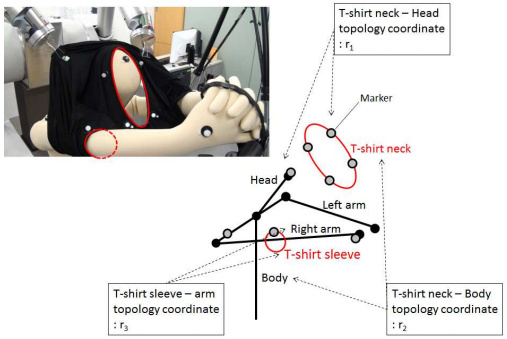
\includegraphics[height=2.5cm]{tamei_2011}
			}
		\end{column}
	\end{columns}
				
	\addtocounter{footnote}{-1}
	\footcitetext{cusumano2011bringing}
	\stepcounter{footnote}
	\footcitetext{tamei2011reinforcement}
\end{frame}

\section{Dynamic Movement Primitives}
\begin{frame}{Dynamic Movement Primitives (DMP)}
	%\linespread{0.8}
	Used for generating control signal to guide real system\footnotemark
	\begin{exampleblock}{Why DMP?}
		\begin{itemize}
			\item A \textit{non-linear} dynamical system used for policy parameterization
			\item Can adapt to complex motor-skills
			\item Also perform target tracking and obstacle avoidance
		\end{itemize}
	\end{exampleblock}
				
	The system is defined as
	\vskip -1em
	\begin{equation*}
		\ddot{y} = \alpha \left( \beta \left(g - y\right) - \dot{y}\right) + f
		\label{eq:attractor_with_f}
	\end{equation*}
	%\begin{equation*}
	%	\ddot{y} = \alpha_y ( \beta_y (g - y) - \dot{y}) + f
	%	\label{eq:attractor_with_f}
	%\end{equation*}
	\vskip -0.5em
	{\small
		where:
		\vskip -0.6em
		\begin{itemize}
			\itemsep0.1em
			\item $y$ is system state and $g$ is goal state
			\item $\alpha$ and $\beta$ are gain terms
			\item $f$ is nonlinear function defined over time
		\end{itemize}
	}
	\vskip -0.6em
	\begin{exampleblock}{}
		$f$ is a function of \textit{canonical system}%, denoted by $x$ as $\dot{x} = -\alpha_x x$
	\end{exampleblock}
				
	\vskip -0.6em
	\footcitetext{schaal2006dynamic}
\end{frame}

\begin{frame}{Forcing function $f$}
	$f$ is defined as
	\vskip-2.8em
	\begin{equation*}
		f(x,g) = \frac{\Sigma_{i=1}^N \psi_i w_i}{\Sigma_{i=1}^N \psi_i} x(g - y_0)
		\label{eq:cs_with_f}
	\end{equation*}
	\vskip -0.5em
	{\small
		where:
		%\vskip-0.8em
		\begin{itemize}
			\setlength\itemsep{0.2em}
			\item $y_0$ is the initial state of the system
			\item $w_i$ is a weighting for a given basis function $\psi_i$
			\item $\psi_i = \textrm{exp}\left( -h_i \left( x - c_i\right)^2 \right)$ is Gaussian with mean $c_i$ and variance $h_i$
		\end{itemize}
	}
	\vskip -1em
	\begin{exampleblock}{Imitating a desired path}
		The desired forcing term $f$ which affects the system acceleration, is written as
		\vskip -1em
		\begin{equation*}
			\textbf{f}_d = \ddot{\textbf{y}}_d - \alpha_y ( \beta_y (g - \textbf{y}) - \dot{\textbf{y}})
			\label{eq:imitate_f}
		\end{equation*}
				
		Choose the weights over the basis functions i.e., minimize\footnotemark
		\vskip -1em
		\begin{equation*}
			\Sigma_t \psi_i(t) \left[ f_d(t) - w_i \left\lbrace x(t) (g - y_0)\right\rbrace\right]^2
			\label{eq:minize_fd}
		\end{equation*}
	\end{exampleblock}
	\vskip -1.5em
	\footcitetext{schaal2002scalable}
\end{frame}

\begin{frame}{Example of DMP}
	\vskip -2em
	\begin{figure}
		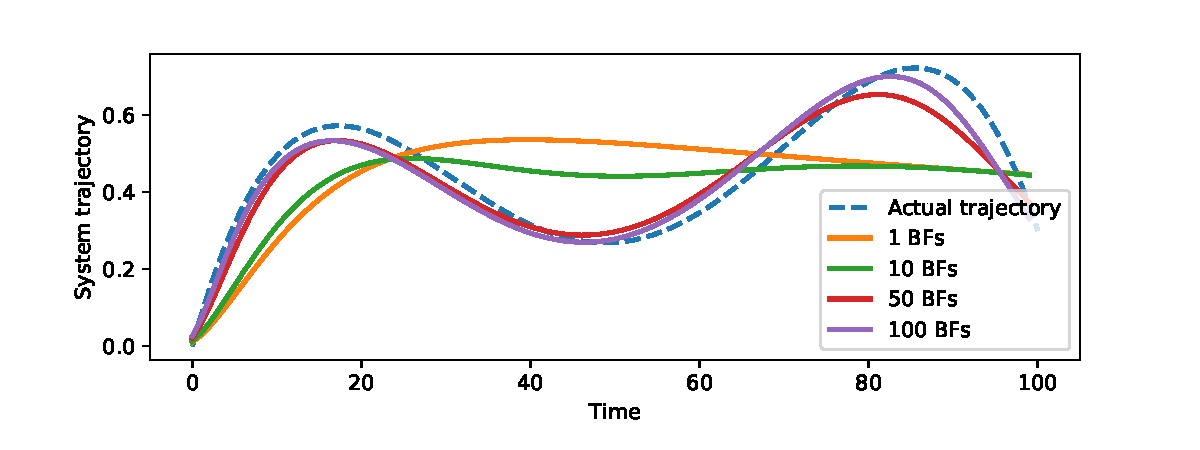
\includegraphics[trim={0 15px 0 0},clip, width=0.9\textwidth]{DMP_BFs}
		\caption{\small{Effect of \textit{no. of basis functions}}}
	\end{figure}
	
	\vskip -2em
	\begin{figure}
		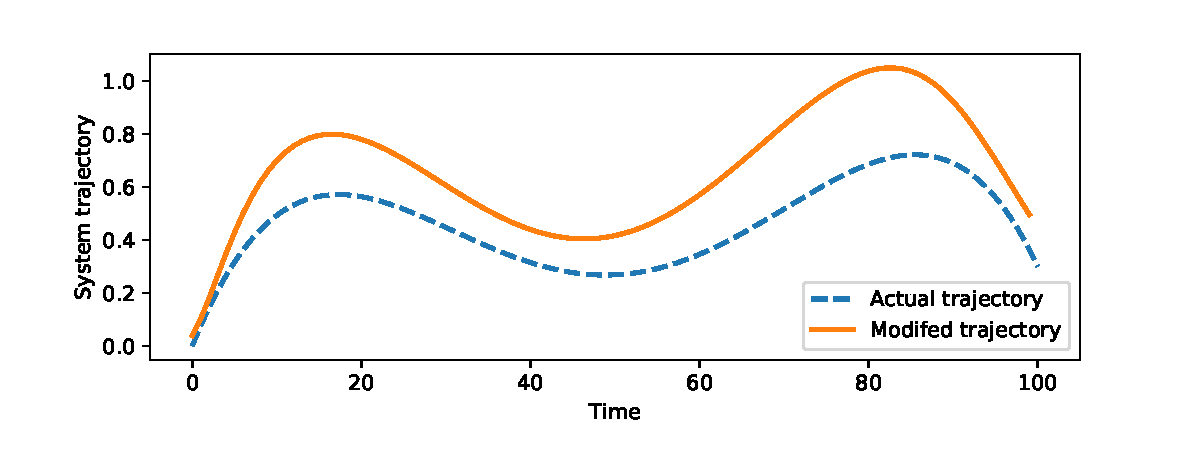
\includegraphics[trim={0 14px 0 20px},clip, width=0.9\textwidth]{DMP_Goal}
		\caption{\small{DMP adaptation to new goal \textit{(new goal = 1.5 * old goal)}}}
	\end{figure}
\end{frame}

\section{Setup and Experiment}
\begin{frame}{Workflow of \textit{Robotic cloth manipulation} task}
	\vskip -0.5em
	\begin{figure}
		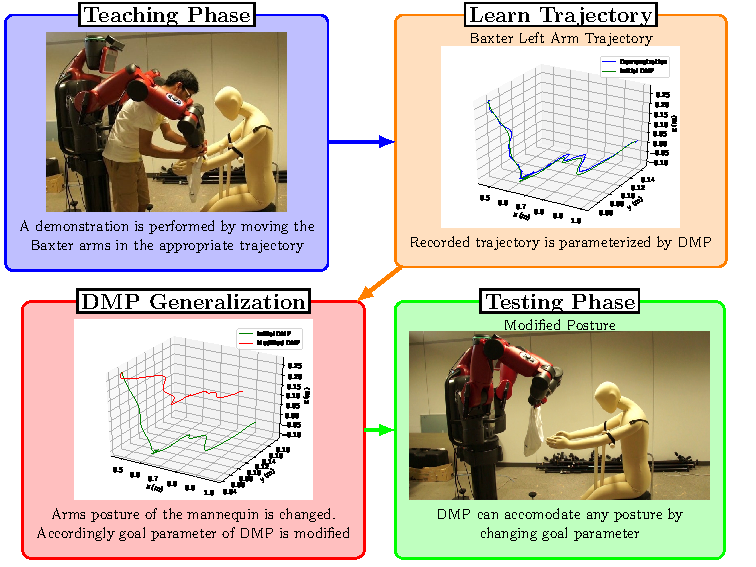
\includegraphics[width=0.9\textwidth]{flowchart_beamer}
	\end{figure}
\end{frame}

\begin{frame}{Setup}
	\begin{figure}
		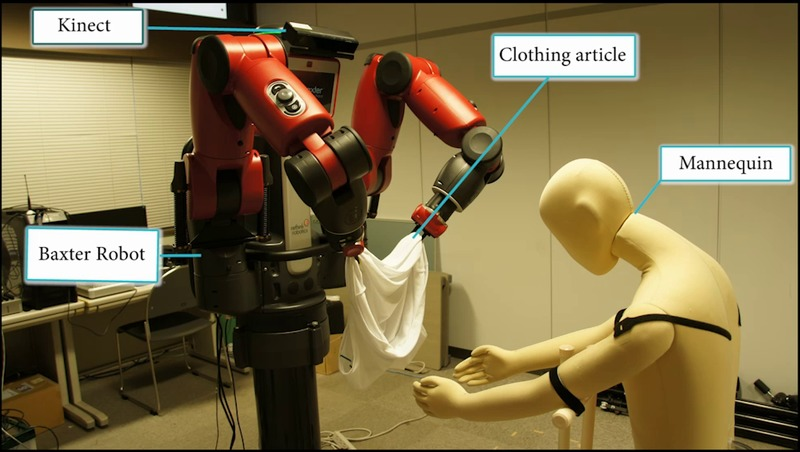
\includegraphics[width=\textwidth]{setup}
	\end{figure}
\end{frame}

\section{Experiments and Results}
\begin{frame}{Experiments and Results}
	\begin{columns}[b]
		\begin{column}{0.5\textwidth}
			\begin{figure}
				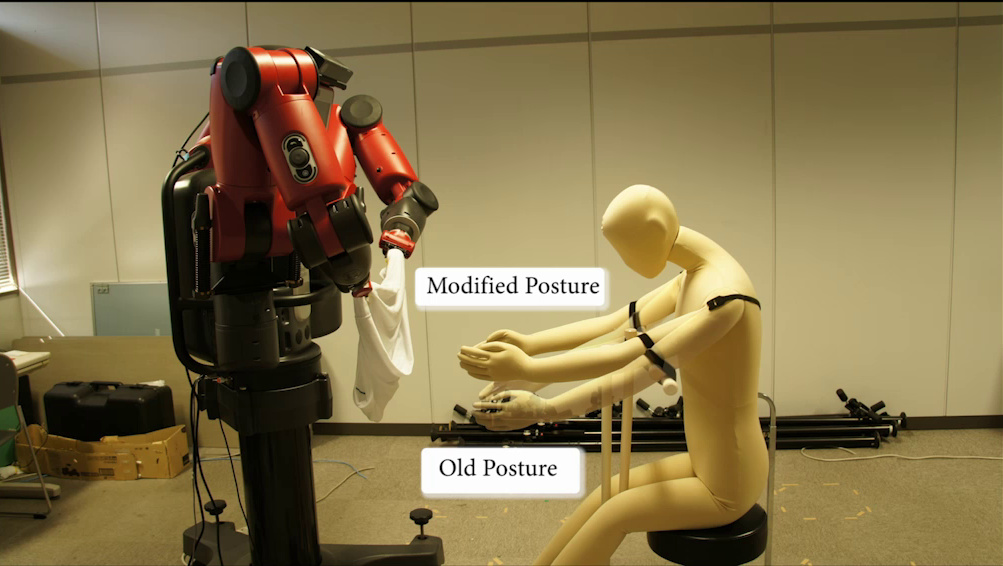
\includegraphics[trim={4cm 0 5cm 0},clip,width=\textwidth]{various_posture}
				\caption{Old \& modified posture of mannequin}
			\end{figure}
		\end{column}
								
		\begin{column}{0.5\textwidth}
			\begin{figure}
				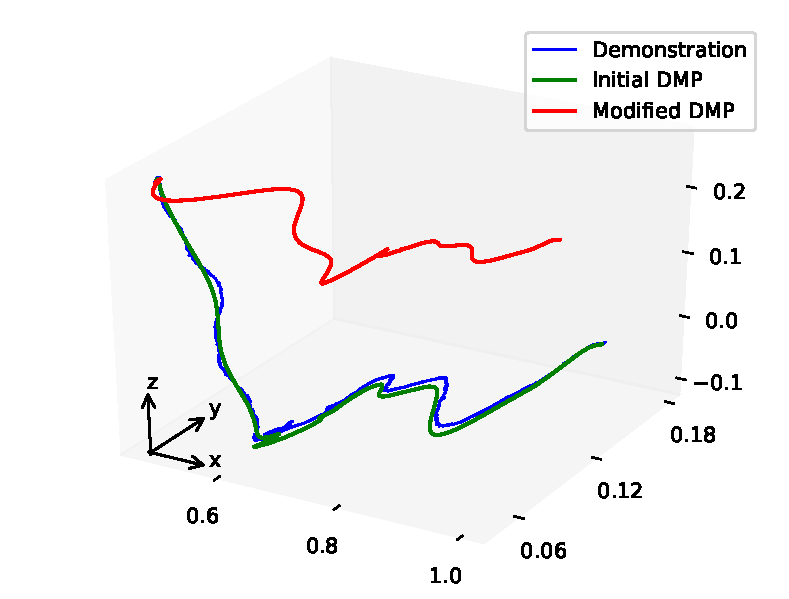
\includegraphics[width=\textwidth]{all_traj}
				\caption{Left arm trajectories of Baxter Robot}
			\end{figure}
		\end{column}
	\end{columns}
				
	\vskip 1em
	\centering{
		\href{run:./videos/video.mp4}{\beamerbutton{Video Demonstration}}
	}
\end{frame}

\begin{frame}{Accuracy measurement}
	Angle of Inclination measures the bending of arms w.r.t. horizontal line in two-dimensional space
	\begin{columns}[t]
		\begin{column}{0.4\textwidth}
			\begin{figure}
				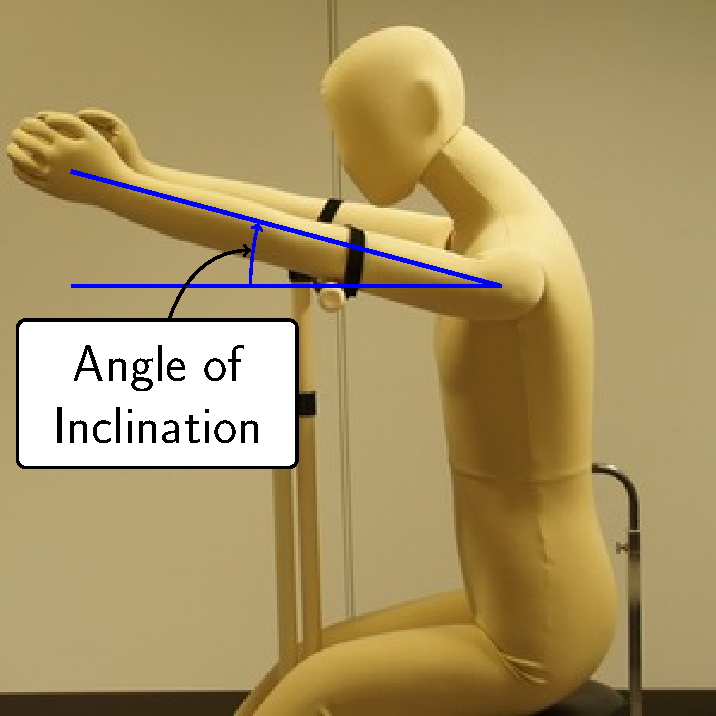
\includegraphics[width=\textwidth]{inclination_plus}
			\end{figure}
		\end{column}
								
		\begin{column}{0.5\textwidth}
			\begin{figure}
				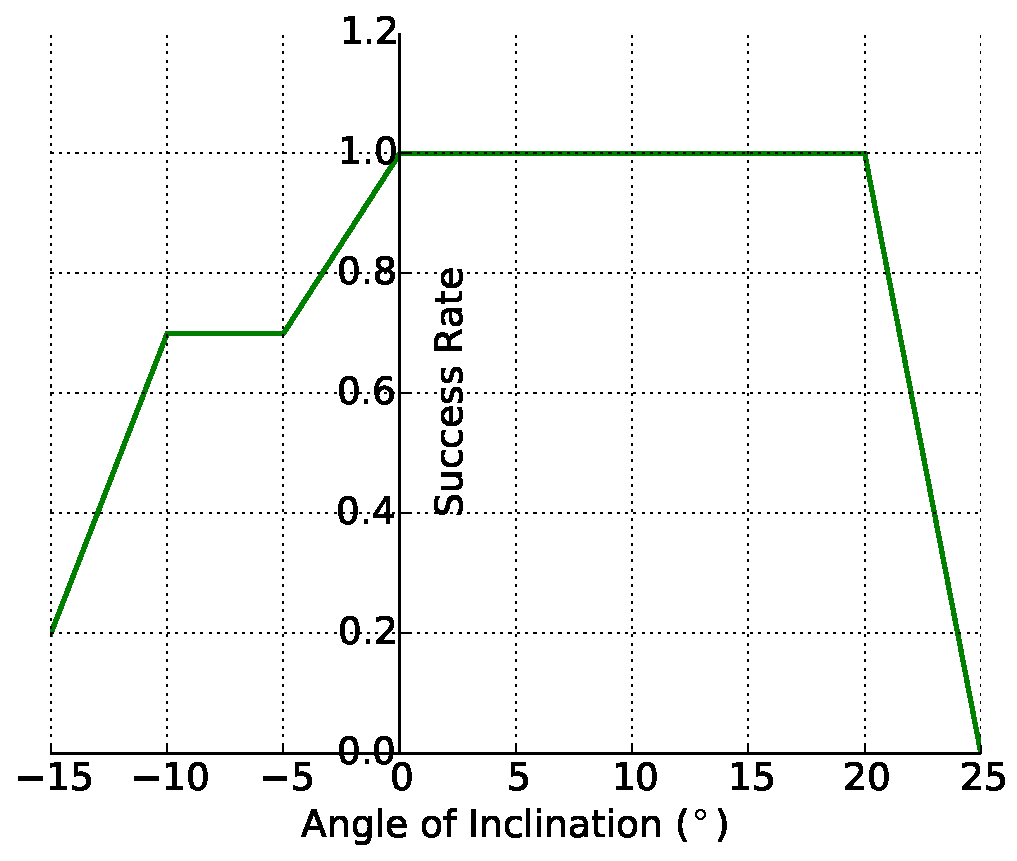
\includegraphics[width=\textwidth]{success_rate}
			\end{figure}
		\end{column}
	\end{columns}
\end{frame}

\section{Discussion and Conclusion}
\begin{frame}{Discussion and Conclusion}
	\linespread{1.5}
				
	\begin{itemize}
		\item Robotic clothing assistance is challenging since it requires cooperative manipulation
		\item Clothing article inherits non-rigid and highly deformable properties
		\item Result shows that DMPs are able to generalize the movement trajectory
		\item DMP should incorporate orientation information as well
	\end{itemize}
\end{frame}

\section{Future work}
\begin{frame}{Future work}
	\linespread{1.5}
				
	\begin{itemize}
		\item Make approach more robust by using combination of visual and force information
		\item Need for designing an adaptive controller
		      \begin{itemize}
		      	\item For real-time tracking of mannequin
		      	\item To adapt various failure scenarios
		      \end{itemize}
	\end{itemize}
				
	\begin{exampleblock}{Acknowledgments}
		This work was supported in part by the Grant-in-Aid for Scientific Research from Japan Society for the Promotion of Science (No. 16H01749).
	\end{exampleblock}
\end{frame}

\begin{frame}[noframenumbering]{References}
	\nocite{*}
	\hspace*{0.5cm}
	\begin{minipage}{\dimexpr\textwidth-1cm\relax}
		\printbibliography
	\end{minipage}
\end{frame}

\begin{frame}[noframenumbering]{The End}
	\begin{center}
		\Huge Thanks for your attention!
		\vskip 1em \huge Any questions?
		\vskip 2em \normalsize \url{www.ravijoshi.xyz}
	\end{center}
	\centering{\hyperlink{supplemental}{\beamerbutton{supplemental here}}}
\end{frame}

\appendix
\section{More}
\begin{frame}[noframenumbering,label=supplemental]
	\frametitle{Dynamic Movement Primitives (DMP)}
	\linespread{1.2}
										
	\begin{exampleblock}{DMP in a nutshell}
		\begin{itemize}
			\item A method of trajectory control/planning\footnotemark
			\item Complex movements are considered as composed of sets of primitive action ‘building blocks’
			      \begin{itemize}
			      	\item Executed in sequence \textit{and/or} in parallel
			      	\item DMPs are a proposed mathematical formalization of these primitives.
			      \end{itemize}
			\item It can represent \textit{nonlinear} motion with a set of differential equations
			\item These equations can be adapted to generate any movement trajectory
		\end{itemize}
	\end{exampleblock}
		
	\footnotetext{\tiny Schaal, Stefan. ``Dynamic movement primitives-a framework for motor control in humans and humanoid robotics." Adaptive Motion of Animals and Machines.  Springer Tokyo, 2006. 261-280.}
\end{frame}

\begin{frame}[noframenumbering]{Formulation of DMP}
	\linespread{1.2}
										
	\textit{DMP is for generating a control signal to guide the real system}
										
	\begin{alertblock}{Underlying Idea\footnotemark}
		\begin{enumerate}
			\item Take a dynamical system with well specified stable behaviour
			\item Add another term that makes it follow some interesting trajectory
		\end{enumerate}
	\end{alertblock}
		
	\vskip 1em			
	There are two kinds of DMP:
	\vskip -0.5em
	\begin{columns}
		\begin{column}{0.5\textwidth}
			\begin{center}
				\textsc{Discrete} DMP
				\vskip -0.5em
				\begin{figure}
					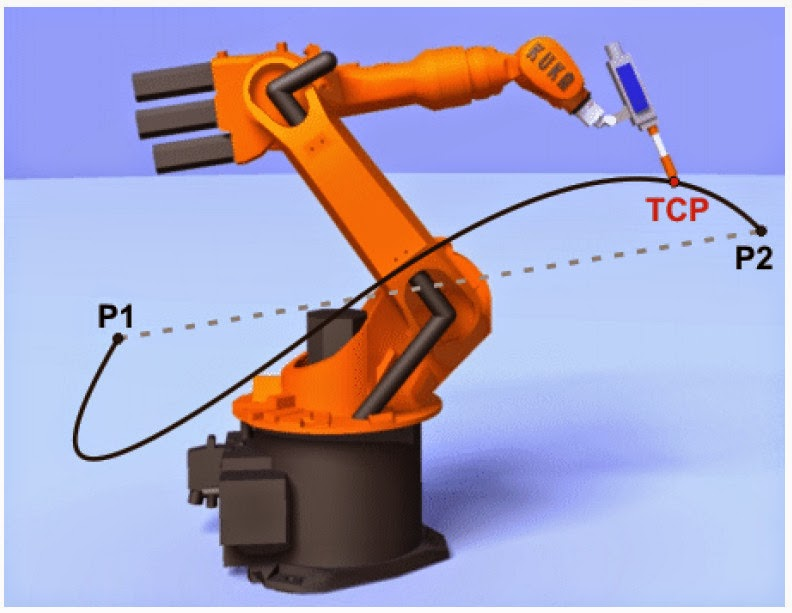
\includegraphics[height=2cm]{images/ptp_motion}
					\vskip -0.5em
					\caption{Point to Point Motion}
				\end{figure}
			\end{center}
		\end{column}
				
		\begin{column}{0.5\textwidth}
			\begin{center}
				\textsc{Rhythmic} DMP
				\vskip -0.5em
				\begin{figure}
					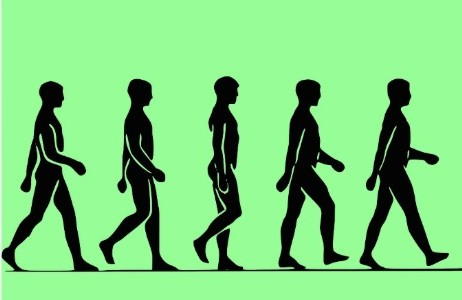
\includegraphics[height=2cm]{images/human_locomotion}
					\vskip -0.5em
					\caption{Human Walking}
				\end{figure}
			\end{center}
		\end{column}
	\end{columns}
									
	\footnotetext{\tiny Ijspeert, A. J., J. Nakanishi, and S. Schaal. ``Learning control policies for movement imitation and movement recognition." Neural information processing system. Vol. 15. 2003.}
\end{frame}

\begin{frame}[noframenumbering]{Formulation of DMP}
	Let's start with point attractor dynamics\footnote{\tiny Ijspeert, Auke Jan, Jun Nakanishi, and Stefan Schaal. ``Movement imitation with nonlinear dynamical systems in humanoid robots." Robotics and Automation, 2002. Proceedings. ICRA'02. IEEE International Conference on. Vol. 2. IEEE, 2002.}
		
	\vskip -1em
	\begin{equation}
		\ddot{y} = \alpha_y ( \beta_y (g - y) - \dot{y})
		\label{eq:attractor}
	\end{equation}
	\vskip -0.5em
	where:
	\begin{itemize}
		\item $y$ is system state and $g$ is goal state
		\item $\alpha$ and $\beta$ are gain terms
	\end{itemize}
				
	\vskip 1em
	Now add a forcing term $f$ on eq(\ref{eq:attractor}) that will let us to modify this trajectory
	\begin{equation}
		\ddot{y} = \alpha_y ( \beta_y (g - y) - \dot{y}) + f
		\label{eq:attractor_with_f}
	\end{equation}
	$f$ is nonlinear function defined over time.
													
	\begin{exampleblock}{}
		\begin{itemize}
			\item[*] The introduced system in eq(\ref{eq:attractor_with_f}) is called the \textit{canonical system}.
			\item[*]  It is denoted by $x$ as $\dot{x} = -\alpha_x x$
		\end{itemize}
	\end{exampleblock}
\end{frame}

\begin{frame}[noframenumbering]{Formulation of DMP}
	The forcing function $f$ is defined as a function of the canonical system:
	\begin{equation}
		f(x,g) = \frac{\Sigma_{i=1}^N \psi_i w_i}{\Sigma_{i=1}^N \psi_i} x(g - y_0)
		\label{eq:cs_with_f}
	\end{equation}
	\vskip -1.0em
	where:
	\begin{itemize}
		\item $y_0$ is the initial state of the system
		\item $w_i$ is a weighting for a given basis function $\psi_i$
		\item $\psi_i = \textrm{exp}\left( -h_i \left( x - c_i\right)^2 \right)$ is Gaussian with mean $c_i$ and variance $h_i$
	\end{itemize}
	\begin{alertblock}{}
		\small Forcing function $f$ is a set of Gaussians that are \textit{activated} as the canonical system $x$ converges to its target.
	\end{alertblock}
				
	\vskip -0.5em
	\begin{columns}
		\begin{column}{0.5\textwidth}
			\begin{figure}
				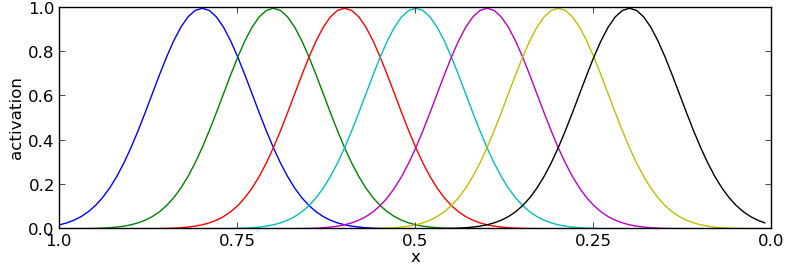
\includegraphics[height=2cm]{images/psi_activation}
				\vskip -0.5em
				\caption{$\psi$ Activation}
			\end{figure}
		\end{column}
				
		\begin{column}{0.5\textwidth}
			\begin{figure}
				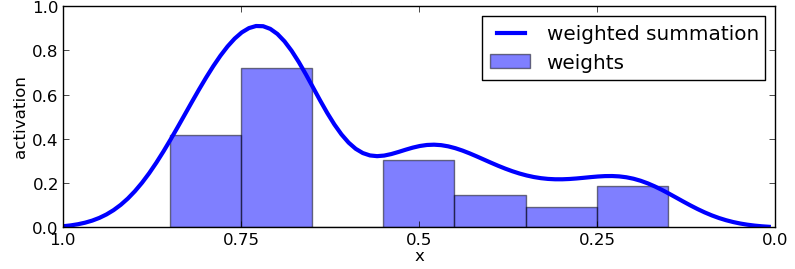
\includegraphics[height=2cm]{images/weighted_summation}
				\vskip -0.5em
				\caption{Weighted Summation}
			\end{figure}
		\end{column}
	\end{columns}
\end{frame}

\begin{frame}[noframenumbering]{Imitating a desired path}
	\linespread{1.4}
	The forcing term $f$ which affects the system acceleration, can be re-written as
	\begin{equation}
		\textbf{f}_d = \ddot{\textbf{y}}_d - \alpha_y ( \beta_y (g - \textbf{y}) - \dot{\textbf{y}})
		\label{eq:imitate_f}
	\end{equation}
	where
	\begin{itemize}
		\item $\textbf{y}_d$ is desired trajectory, given by $\ddot{\textbf{y}}_d = \frac{\partial}{\partial t} \dot{\textbf{y}}_d = \frac{\partial}{\partial t} \frac{\partial}{\partial t} \textbf{y}_d$
	\end{itemize}
															
	\begin{exampleblock}{Forcing term}					
		\begin{itemize}
			\item Comprised of weighted summation of basis functions
			\item We can use optimization technique like LWR\footnotemark
			      \begin{itemize}
			      	\item[*] To choose the weights over our basis functions
			      	\item[*] Minimize
			      	      \vskip -2em
			      	      \begin{equation}
			      	      	\Sigma_t \psi_i(t)(f_d(t) - w_i (x(t) (g - y_0)))^2
			      	      	\label{eq:minize_fd}
			      	      \end{equation}
			      \end{itemize}
		\end{itemize}
	\end{exampleblock}
					
	\footnotetext{\tiny Cleveland, William S. ``Robust locally weighted regression and smoothing scatterplots." Journal of the American statistical association 74.368 (1979): 829-836.}
\end{frame}

\begin{frame}[noframenumbering]{Imitating a desired path}
	The solution\footnote{\tiny Schaal, Stefan, Christopher G. Atkeson, and Sethu Vijayakumar. ``Scalable techniques from nonparametric statistics for real time robot learning." Applied Intelligence 17.1 (2002): 49-60.} of eq(\ref{eq:minize_fd}) $w_i = \frac{\textbf{s}^T \pmb{\psi}_i \textbf{f}_d}{\textbf{s}^T \pmb{\psi}_i \textbf{s}}$	\\
	where
	\begin{itemize}
		\item[] $\textbf{s} = \left( \begin{array}{c}x_{t_0}(g - y_0) \\ \vdots \\ x_{t_N}(g - y_0) \end{array} \right)$ and $\pmb{\psi}_i = \left( \begin{array}{ccc} \psi_i(t_0) & \dots & 0 \\ 0 & \ddots & 0 \\ 0 & \dots & \psi_i(t_n) \end{array} \right)$
	\end{itemize}
				
	\begin{figure}
		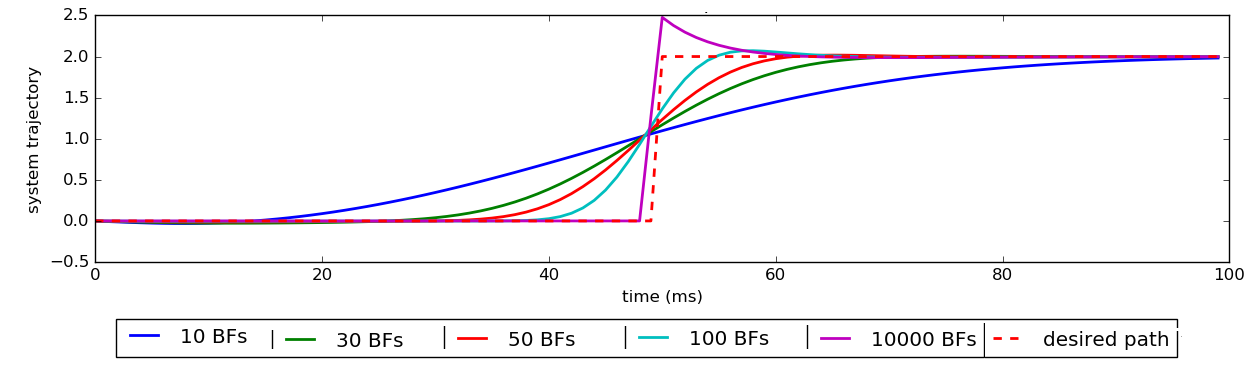
\includegraphics[width=0.9\textwidth]{images/imitate_path}
	\end{figure}
	\vskip -0.7em
	%\centering{
	\tiny{Back to \hyperlink{main}{\beamerbutton{main}}}
	%}
\end{frame}
\end{document}
